\documentclass[a4paper,12pt]{article}

% Packages
\usepackage{animate}
\usepackage{amsmath}
\usepackage{amssymb}
\usepackage{bibentry}
\usepackage{color}
\usepackage{dirtree}
\usepackage{geometry}
\usepackage{graphicx}
\usepackage{hyphenat}
\usepackage{indentfirst}
\usepackage{listings}
\usepackage{ipsum}
\usepackage{titlesec}
\usepackage{url}
\usepackage{physics}
\usepackage{fontspec}
\usepackage[normalem]{ulem}
\usepackage[backend=biber, style=apa]{biblatex}
\usepackage[
colorlinks=true,
linkcolor=blue,
urlcolor=cyan,
citecolor=blue,
breaklinks=true,
]{hyperref} % For hyperlinks

\definecolor{dkgreen}{rgb}{0,0.6,0}
\definecolor{gray}{rgb}{0.5,0.5,0.5}
\definecolor{mauve}{rgb}{0.58,0,0.82}
\setmonofont{CaskaydiaCove Nerd Font}
\lstset{
	aboveskip=3mm,
	basicstyle=\ttfamily\small,
	belowskip=3mm,
	breakatwhitespace=true,
	breaklines=true,
	columns=flexible,
	commentstyle=\color{dkgreen},
	frame=none,
	keywordstyle=\color{blue},
	language=C++,
	numbers=none,
	numberstyle=\tiny\color{gray},
	showstringspaces=false,
	stringstyle=\color{mauve},
	tabsize=4
}
\addbibresource{references.bib}
\geometry{margin=1in}
\titleformat{\chapter}[display]
{\normalfont\huge\bfseries}{\chaptertitlename\ \thechapter}{20pt}{\Huge}
\titlespacing{\chapter}{0pt}{0pt}{0pt}
\sloppy

% Title and Author
\title{Computational Fluid Dynamics With a Paper Airplane}
\author{
  Tasada, Daniel\\
  \and
  Tse, Nathan\\
}
\date{\today}

\begin{document}

% Title and abstract
\maketitle
\begin{abstract}
	In this paper, we investigate the relationship between an airplane's shape
	and its performance. Our results show that \dots
\end{abstract}

% Table of Contents
\tableofcontents

% Introduction
\section{Introduction}
This thesis covers the simulation of the aerodynamics of an airplane, using
our own Computational Fluid Dynamics model (CFD).

The goal is to simulate the airflow around an airplane's body. CFD is a
branch of fluid mechanics that uses numerical methods and algorithms to solve
and analyze problems that involve fluid flows. It is used in many fields,
including aerospace engineering, automotive engineering, and meteorology.

The application of CFD to an airplane is important because it allows testing
of a model's aerodynamic performance without building a physical model, or
have to set up a wind tunnel. The practical alternative is much more expensive
and time-consuming.

The final aim is to determine how the shape of an airplane's body affects its
performance. Part of the project is to dynamically generate 3D models of
airplanes, and simulate the airflow around them. The intention is to use
machine learning to optimize the shape of the airplane's body to maximize
performance.

CFD is challenging in the sense that it requires a good understanding of fluid
dynamics, as well as a good understanding of the math involved. CFD is also
very expensive from a computational perspective, so code optimization is important.

The thesis questions are the following:
\begin{itemize}
	\item{How do the different aspects of fluid dynamics work and how do we
		implement it in a computer program?}
	\item{How do we dynamically generate 3D models?}
	\item{How does an airplane's wing shape influence its performance?}
\end{itemize}

% Execution
\section{Execution}
\subsection{Preliminary: Lagrangian Fluid Simulation}
One method of simulating fluid dynamics is the Lagrangian method. This method
models the fluid as a particle collision system, where the air is represented by
particles that interact with each other to emulate a fluid. Our implementation
is based on \hyperlink{http://www.hakenberg.de/diffgeo/collision_resolution.htm}{Rigid Body Collision Resolution}
(\cite{hakenberg}). We used this paper as a guide for all the math involved.

The math relies on the momentum, inertia, and velocity of the particles to
calculate the collision normal and point of contact. The collision normal is
the direction in which the particles are moving away from each other, and the
point of contact is the point at which the particles collide.

The following variables are necessary to perform the calculations:
\[
\begin{array}{ll}
	\text{Angular momentum $L$ } (kg\cdot m^2/s): & L = mvr; \\
	\text{Inertia tensor $I$ } (kg\cdot m^2): & I = \frac{L}{\omega}; \\
    \text{Angular velocity $\omega$ } (rad/s): & \omega = \frac{\Delta \theta}{\Delta t}; \\

	\\

	\text{Collision normal} (n \in \mathbb{R}^3) \text{ in world coordinates away from body}; \\
	\text{Point of contact } (r_i \in \mathbb{R}^3) \text{ in world coordinates with respect to $p_i$}; \\
	\text{Orientation } (R_i \in SO(3)) \text{ transforming from object to world coordinates}; \\
\end{array}
\]

Where $i$ represents one of two particles in a given collision:
\[
\begin{array}{ll}
	\text{Velocity after collision} & \tilde{v}_i, \\ 
	\text{Angular velocity after collision} & \tilde{\omega}_i, \\
	\text{Constant} & \lambda, \\
\end{array}
\]

The following formulas represent the relation between particles:
\[
\begin{array}{cc}
	\tilde{v}_1 = v_1 - \frac{\lambda}{m_1} n; \\ 
	\tilde{v}_2 = v_2 + \frac{\lambda}{m_2} n; \\
	\tilde{\omega}_1 = \omega_1 - \Delta q_1; \\
	\tilde{\omega}_2 = \omega_2 + \Delta q_2; \\

	\text{where } q_i := I_i^{-1} \cdot R_i^{-1} \cdot (r_i\times n), \\
	\text{and } \lambda = 2 \frac{n v_1 - n v_2 + \omega_1 I_1 q_1 - \omega_2 I_2 q_2}
	{(\frac{1}{m_1} + \frac{1}{m_2})n^2 + q_1 I_1 q_1 + q_2 I_2} \\
\end{array}
\]

This was implemented using Go and raylib, and the code is available at
\href{www.github.com/dtasada/paper}{github.com/dtasada/paper} at the \lstinline{lagrangian-go} branch.

When dealing with a lot of particles, the simulation stops performing as well,
because the number of calculations and iterations of the formulas listed above
has a time complexity of $O(n^2)$, where $n$ is the number of particles. This is
because every particle handles collisions with every other particlee every
single frame. This can be elegantly mitigated by implementing a three-dimensional
grid system, where every particle is assigned to a cell in the grid. This way,
particles only need to check for collisions with other particles in the same cell
or neighboring cells. If the particles are evenly distributed within the container,
each particle only needs to handle collisions with particles in its own cell, and
its 26 neighboring cells. This reduces the time complexity to $O(n)$.

The simulation was unstable at higher densities, where particles would phase
into each other instead of cleanly bouncing. The bug is likely quite simple to
fix, but we got distracted by another method. Despite the optimizations we
made, Lagrangian simulation is still quite computationally expensive, and Go
probably wasn't doing it any favors (Go isn't very memory efficient). In the
end it was put aside, and the Lagrangian implementation was never completed.

\subsection{Eulerian Fluid Simulation}
The other method is the Eulerian method. This method models the fluid as a
cellular automata. The fluid is represented by a grid of cells, each of which
has its own properties and interacts with its neighbor cells, creating a mesh.

Our fluid simulation involves a three-dimensional grid of cells, each of which
have velocity and density fields. Each frame, the cells interact with each
other according to the \href{https://en.wikipedia.org/wiki/Navier%E2%80%93Stokes_equations}{Navier-Stokes equations}.

The specific math involved in the base equations for the fluid simulation is
quite complex, and we couldn't have derived it on our own, so we used
Mike Ash's implementation \href{www.mikeash.com/pyblog/fluid-simulation-for-dummies.html}{\citefield{mikeash}{title}} (\cite{mikeash})
as the bedrock of our program. Mike Ash's  which is in turn based on Jos Stam's
brilliant work on \href{www.dgp.toronto.edu/public_user/stam/reality/Research/pdf/GDC03.pdf}{\citefield{josstam}{title}} (\cite{josstam}).

% Math
\subsubsection{The Math}
In Eulerian fluid dynamics we represent fluids with a velocity vector field. This means we assign a velocity vector to every point in space.
The Navier-Stokes equations show us how these velocity vectors evolve over time with an infinitely small timestep.
\[
	\begin{array}{ll}
		\pdv{u}{t} = -(u \cdot \nabla)u + v\nabla^2 + f \\
		\\
		\pdv{\rho}{t} = -(u \cdot \nabla)\rho + k\nabla^2\rho + S
	\end{array}
\]
The first equation shows the change in velocity in a compact vector notation. 
Unlike in Lagrangian fluid simulation, in Eularian fluid simulation the fluid is not represented by individual particles. 
Thats why, instead, fluid density is used, which tells us the amount of particles present in a point in space. 
The second equation represents the change of this density. 
The reader is not expected to fully understand these equations because they are, as mentioned earlier,
very difficult to understand. But it should be noted that the two equations above look a lot like eachother,
as this was helpful in developing the simulation. (\cite{josstam})

\subsubsection{The Implementation}
Our code is structured as follows:
\dirtree{%
	.1 paper.
	.2 neural\DTcomment{Contains ML engine}.
	.2 simulation/\DTcomment{Contains the physics simulation code}. 
	.3 include/\DTcomment{Our own engine headers}.
	.3 resources/\DTcomment{Resources like images, fonts, shaders}.
	.3 src/\DTcomment{Actual engine source}.
	.3 config.toml\DTcomment{Configuration file}.
	.3 Makefile.
}

This codebase is written in C++, and uses the \hyperlink{https://www.raylib.com/}{raylib}
because it's a really simple and powerful library that allows us to focus on the
simulation itself, as it provides a bunch of tools to easily render 3D graphics.
The reason this codebase is in C++ was initially because we never got the Eulerian
model to work in Go, likely due to a mistake of our own. Nevertheless we think C++
was the right choice, as it's more appropriate for the vector physics and low overhead
we need for the simulation.

The main class we use for the simulation is the \verb|Fluid| class. The implementation
is available at \verb|/simulation/src/Fluid.cpp|. The interface is as follows: \\
\begin{center}
	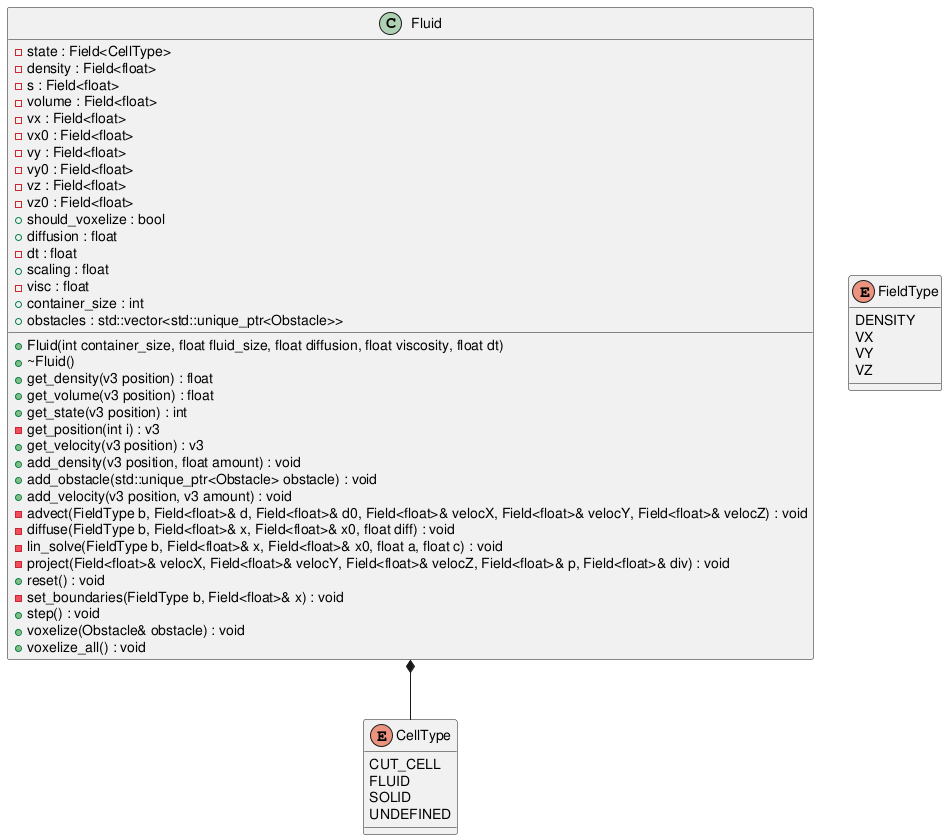
\includegraphics[width=\textwidth]{resources/Fluid.png}
\end{center}

The class contains the cell property fields as well as all the functions related
to the physics simulation, including the advection, diffusion and projection procedures.
With this we have a basic working fluid simulator.

The next step is to add geometry. We did this by adding a boolean field to the
Fluid properties and some getters and setters.
\begin{lstlisting}
class Fluid {
   private:
	// rest of private members
	bool *solid;

   public:
	// rest of public members
	bool is_solid(v3 position);
	void set_solid(v3 position, bool set);
}
\end{lstlisting}
Then we change the advection and boundary handling functions to account for
solid boundaries. This is done by checking whether each cell is solid, and if
so, the cell properties aren't advected.

\begin{lstlisting}
// in advection function, for each cell:
if (solid[IX(i, j, k)]) {
	if (b != FieldType::DENSITY) {  // For velocity components
		d[IX(i, j, k)] = 0;
	}
	continue;
}

// in boundary function, for each cell:
if (solid[IX(x, y, z)]) {
	// For velocity components, enforce no-slip condition
	if (b == FieldType::VX) f[IX(x, y, z)] = 0;  // x velocity
	if (b == FieldType::VY) f[IX(x, y, z)] = 0;  // y velocity
	if (b == FieldType::VZ) f[IX(x, y, z)] = 0;  // z velocity

	// For density and pressure, use average of neighboring
	// non-solid cells
	if (b == FieldType::DENSITY) {
		float sum = 0;
		int count = 0;

		if (!solid[IX(x-1, y, z)]) { sum += f[IX(x-1, y, z)]; count++; }
		if (!solid[IX(x+1, y, z)]) { sum += f[IX(x+1, y, z)]; count++; }
		if (!solid[IX(x, y-1, z)]) { sum += f[IX(x, y-1, z)]; count++; }
		if (!solid[IX(x, y+1, z)]) { sum += f[IX(x, y+1, z)]; count++; }
		if (!solid[IX(x, y, z-1)]) { sum += f[IX(x, y, z-1)]; count++; }
		if (!solid[IX(x, y, z+1)]) { sum += f[IX(x, y, z+1)]; count++; }

		f[IX(x, y, z)] = count > 0 ? sum / count : f[IX(x, y, z)];
	}
}
\end{lstlisting}

This allows us to add a cube of a given size at a given position, which the
fluid will treat as a solid object. Unfortunately, a plane is more complex than
a cube. There are a few ways to handle this. The most obvious and least efficient
is to raise the resolution of the grid. Currently we've been experimenting with a
24x24x24 or a 32x32x32 grid, and that's already not as performant as we'd like.
A 24x24x24 grid has to iterate $24^3 = 13824$ times per frame. And to simulate
complex shapes, the higher resolution the better. But simply increasing the
resolution to something like 128x128x128 or higher just isn't viable.

We're still implementing this at the time of writing the concept, but the goal
is to use the method explained above in combination with the Cut-Cell method,
which will dynamically create more of these cells along the borders of the model,
in this case a plane. This would create a high-resolution grid near the important
and complex areas of the simulation, while preserving resources by keeping the
unimportant areas (like large patches of just air) from being computed.

% Results
\section{Results}
\ipsum[1]

% Conclusion
\subsection{Conclusion}
\ipsum[1]

% References
\nocite{*}
\printbibliography

\end{document}
